\begin{frame}[c]
  \frametitle{Time series data}
  
\begin{center}
  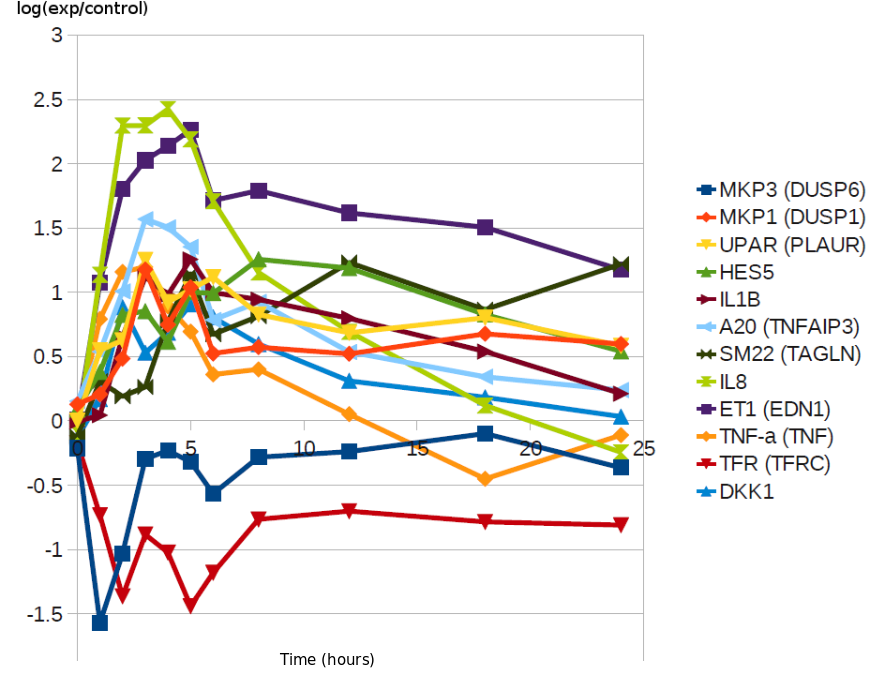
\includegraphics[width=70mm]{figs/12genes.png}
\end{center}

%\pause

\begin{columns}
\begin{column}{0.7\textwidth}
\begin{itemize}
  \item Experiment: \tval{calcium stimuli}
  \item Measured at 10 time-points(0-24hrs)
  \item \tval{$200$ transcripts} selected  (\tval{dynamic patterns}) %their fold expression with respect to the non-stimulated cell was significant in at least one time point
  \item We included in our model a subset of $12$ of them
\end{itemize}
\end{column}

\begin{column}{0.3\textwidth}
% \textbf{ \small Prof. Dr. Peter Angel
%Signal Transduction and Growth Control (A100)
%German Cancer research center
%Heidelberg, Germany}

\end{column}
\end{columns}
%\textcolor{couleurtheme}{$\Rightarrow$} \fbox{\tval{\large Allow efficient translation from Process Hitting to BRN}} \textcolor{couleurtheme}{$\Leftarrow$}

\end{frame}

